%%%%%%%%%%%%%%%%%%%%%%%%%%%%%%%%
% Compile with
% pdflatex --shell-escape -synctex=1 -interaction=nonstopmode rasterGrid.tex
% to convert it to png use:
% convert -density 300 -transparent white "\image.pdf" "\image.png"},
%%%%%%%%%%%%%%%%%%%%%%%%%%%%%%%%

\documentclass{standalone}

\usepackage[utf8]{inputenc}
\usepackage{tkz-fct}
\renewcommand{\familydefault}{\sfdefault}
\usepackage[scaled=1]{helvet}
\usepackage[helvet]{sfmath}
\everymath={\sf}
\usetikzlibrary{calc,arrows,intersections,angles,quotes,patterns}

\definecolor{AFLight}{HTML}{5CE0E6}
\definecolor{AFMiddle}{HTML}{51ADE5}
\definecolor{AFDark}{HTML}{0E4160}

\begin{document}

\tikzset{
   every node/.style={scale=1.3},
   >=stealth
}

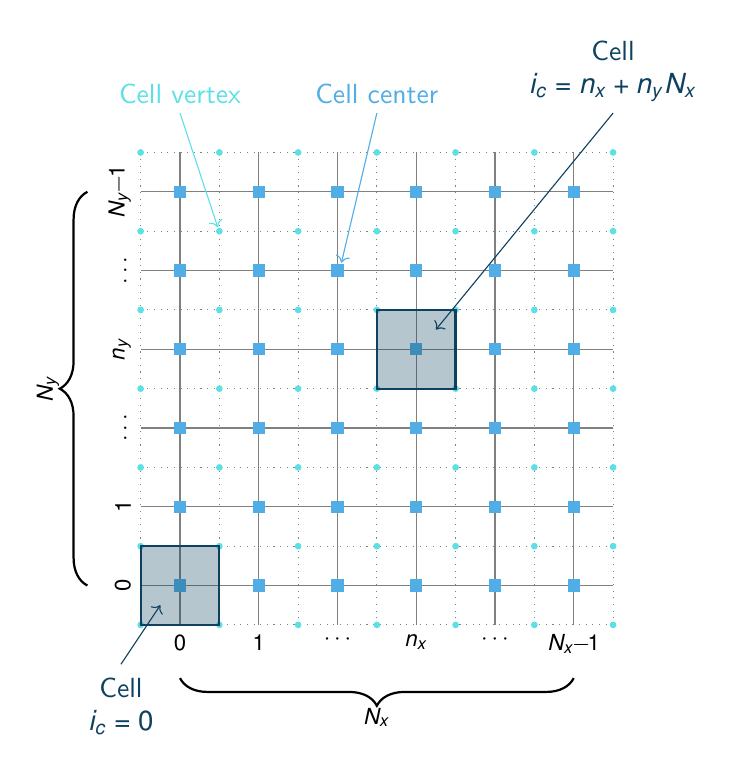
\begin{tikzpicture}[
    scale=1
 ]
 \def\xMin{0}
 \def\xMinSec{1}
 \def\yMin{0}
 \def\yMinSec{1}
 \def\xMax{5}
 \def\yMax{5}

 \def\xxMin{-0.5}
 \def\xxMinSec{0.5}
 \def\yyMin{-0.5}
 \def\yyMinSec{0.5}
 \def\xxMax{5.5}
 \def\yyMax{5.5}
     \foreach \i in {\xMin,\xMinSec,...,\xMax} {
         \draw [gray] (\i,\yMin-0.5) -- (\i,\yMax+0.5);
     }
     \foreach \i in {\yMin,\yMinSec,...,\yMax} {
         \draw [gray] (\xMin-0.5,\i) -- (\xMax+0.5,\i);\foreach \j in {\yMin,\yMinSec,...,\yMax} {
             \draw [color=AFMiddle] plot [only marks, mark size=2, mark=square*] coordinates {(\j,\i)};
         }
     }

     \foreach \i in {\xxMin,\xxMinSec,...,\xxMax} {
         \draw [thin, dotted, gray] (\i,\yyMin) -- (\i,\yyMax);
     }
     \foreach \i in {\yyMin,\yyMinSec,...,\yyMax} {
         \draw [thin, dotted, gray] (\xxMin,\i) -- (\xxMax,\i);
         \foreach \j in {\yyMin,\yyMinSec,...,\yyMax} {
             \draw [color=AFLight] plot [only marks, mark size=1, mark=*] coordinates {(\j,\i)};
         }
     }

 \draw (0,\yMin-0.5) node[below] {\footnotesize $0$};
 \draw (1,\yMin-0.5) node[below] {\footnotesize $1$};
 \draw (2,\yMin-0.5) node[below] {\footnotesize $\cdots$};
 \draw (3,\yMin-0.5) node[below] {\footnotesize $n_x$};
 \draw (4,\yMin-0.5) node[below] {\footnotesize $\cdots$};
 %\draw (4,\yMin-0.5) node[below] {\footnotesize $N_{cols}-2$};
 \draw (5,\yMin-0.5) node[below] {\footnotesize $N_{x}\!\!-\!\!1$};


 \draw (\xMin-0.5,0) node[rotate = 90, above] {\footnotesize $0$};
 \draw (\xMin-0.5,1) node[rotate = 90, above] {\footnotesize $1$};
 \draw (\xMin-0.5,2) node[rotate = 90, above] {\footnotesize $\cdots$};
 \draw (\xMin-0.5,3) node[rotate = 90, above] {\footnotesize $n_y$};
 \draw (\xMin-0.5,4) node[rotate = 90, above] {\footnotesize $\cdots$};
 %\draw (4,\yMin-0.5) node[below] {\footnotesize $N_{cols}-2$};
 \draw (\xMin-0.5,5) node[rotate = 90, above] {\footnotesize $N_{y}\!\!-\!\!1$};



 \draw[color=AFDark, thick, fill=AFDark, fill opacity=0.3] (2.5,2.5) rectangle ++(1,1);
 \draw[->, AFDark] (5.5,6) node[above] {\begin{tabular}{c} Cell \\ $i_c = n_x + n_yN_x$ \end{tabular}} -- (3.25,3.25);
 \draw[color=AFDark, thick, fill=AFDark, fill opacity=0.3] (-0.5,-0.5) rectangle ++(1,1);
 \draw[->, AFDark] (-0.75,-1) node[below] {\begin{tabular}{c} Cell \\ $i_c = 0$ \end{tabular}} -- (-0.25,-0.25);

 \draw[->, AFMiddle] (2.5,6) node[above] {Cell center} -- (2.05,4.1);

 \draw[->, AFLight] (0,6) node[above] {Cell vertex} -- (0.48,4.55);


 \draw [thick,decorate,decoration={brace,amplitude=10pt,mirror},yshift=-5pt](\xMin,\yMin-1) -- (\xMax,\yMin-1) node[black,midway,yshift=-0.5cm] {\footnotesize $N_{x}$};
 \draw [thick,decorate,decoration={brace,amplitude=10pt,mirror},xshift=-5pt](\xMin-1,\yMax) -- (\xMin-1,\yMin) node[black,midway,xshift=-0.5cm, rotate = 90] {\footnotesize $N_{y}$};
 \end{tikzpicture}

\end{document}
